\documentclass{article}
    \usepackage{subcaption}
    \usepackage{amsmath, amssymb}
    \usepackage{graphicx, float}
    \usepackage[hidelinks]{hyperref}
    \usepackage[bottom]{footmisc}
    \usepackage[margin=.8in, tmargin=.8in]{geometry}
    \usepackage{esint} % for double line integrals
    \usepackage{xcolor} % for color macros
    \usepackage{tikz}
    \usepackage{algorithm, algpseudocode}
    \newcommand{\citep}[2][]{(\cite[#1]{#2})}

    \usetikzlibrary{arrows,decorations.markings}
    \usepackage[
        backend=biber,
        % style=alphabetic,
        citestyle=authoryear,
        sorting=ynt
    ]{biblatex}
    
    \bibliography{bibliography}

    \renewcommand{\baselinestretch}{1.2}
    \newcommand{\eps}{\epsilon}
    \newcommand{\der}{\partial}
    \newcommand{\del}{\nabla}
    \newcommand{\bm}[1]{\mathbf{#1}}
    % \newcommand{\vf}[1]{\vec{\mathbf{#1}}}
    \newcommand{\vf}[1]{\mathbf{#1}}
    \newcommand{\norm}{\hat{\bm{n}}}
    \newcommand{\normal}{\mathcal{N}}
    \newcommand{\var}{\text{var}}
    \newcommand{\bx}{\vf{x}}
    \newcommand{\by}{\vf{y}}
    \newcommand{\bz}{\vf{z}}
    \newcommand{\bw}{\vf{w}}
    \newcommand{\bfu}{\vf{f}}
    \newcommand{\giv}{\ |\ }
    \newcommand{\bmu}{\pmb{\mu}}
    \newcommand{\gauss}{\mathcal{N}}
    \newcommand{\data}{\mathcal{D}}
    \newcommand{\model}{\mathcal{M}}
    \DeclareMathOperator*{\argmax}{arg\,max}
    \DeclareMathOperator*{\argmin}{arg\,min}

    \newcommand{\id}{\mathbb{I}}
    \newcommand{\de}{\text{d}}
    \newcommand{\tran}{\text{T}}
    \newcommand{\expect}{\mathbb{E}}
    \newcommand{\kl}{D_{KL}}
    \newcommand{\post}{P(\bw \giv \data)}

    \newcommand{\red}[1]{\textcolor{red}{#1}}
    \newcommand{\blue}[1]{\textcolor{blue}{#1}}
    
    \setlength\parindent{0pt}
    \captionsetup{justification=centering}
    
    \title{Machine Learning and Pattern Recognition}
    \date{\today}
    \author{Traiko Dinev \textless traiko.dinev@gmail.com\textgreater}

\begin{document}

\maketitle
\textit{NOTE: This partially follows Machine Learning and Pattern Recognition, a masters level course at the University of Edinburgh.}

\textit{NOTE: Note this "summary" is NOT a reproduction of the course materials nor is it copied from the corresponding courses. It was entirely written and typeset from scratch.}

\textit{License: Creative Commons public license; See README.md of repository}

\section{Linear Regression}
Consider the vector of features $\bm{x} = \langle x_1, x_2, \dots, x_D \rangle$, where $D$ is the number of dimensions. Then we want to learn this transformation (i.e. learn $\bm{w}$):

\begin{equation}
    \bm{f} = X \bm{w} + b
\end{equation}

where X is a $N\times D$ matrix, containing $N$ examples of $D$ dimensions. We have $N$ targets, our training vector $y$ of size $N\times1$. This corresponds to computing $\bm{w}^T \bm{x}^{(i)}$, i.e. the dot product between the weights and training examples for each $i$. We can use mean squared error:

\begin{align*}
    \min_{\bm{w}} \quad& \sum_i (y^{(i)} - f^{(i)})^2
        = (\bm{y} - \bm{f})^T (\bm{y} - \bm{f})
\end{align*}

This has a linear solution of the form $\bm{w} = \underbrace{(X^TX)^{-1}X^T}_\text{\blue{pseudo-inverse}} \bm{y}$. We can also introduce basis functions $phi$:
\vskip 0.1in

\begin{align*}
    f(\bm{x}) &= \sum_k w_k\ \phi_k(\bm{x}) \\
    \phi(\bm{x}) &= \exp(-(\bm{x} - \bm{c})^T (\bm{x} - \bm{c}) / h^2)
        && \text{\blue{Radial Basis Function}} \\
    \sigma(\bm{x}) &= \frac{1}{\exp(-\bm{v}^T \bm{x} - b)}
        && \text{\blue{Sigmoid}}
\end{align*}

\subsection{Regularization}
We can add L2 regularization, which penalizes big weights.

\begin{equation}
    \hat{E}(\bm{w}) = E(\bm{w}) + \lambda \bm{w}^T\bm{w}
\end{equation}

which we can solve analytically to get something similar:

\begin{equation}
    \bm{w}^* = (X^TX + \lambda \id)^{-1}X^T \bm{y}
\end{equation}

Alternatively, we can augment the $\bm{y}$ vector and $X$ matrix to obtain the same results:

\begin{align*}
    \bm{y}' =
        \begin{pmatrix}
            \bm{y} \\
            \bm{0}_k
        \end{pmatrix} \\
    \Phi' =
        \begin{pmatrix}
            \Phi \\
            \sqrt{\lambda} \id_k
        \end{pmatrix}
\end{align*}

\section{Error Bars}
We normally train on a \textit{training set}, find best hyperparameters (like the L2 coefficients) on a \textit{validation set} and judge only once on a \textit{test set}.

Now let's say we compute some error measure or loss $L(y, f(x))$, like the mean squared error above. If we have a test set, we can compute the mean of this error:

\begin{equation}
    L_\text{test} = \frac{1}{M} \sum_{m=1}^M L(y_m, f(x_m)) = \frac{1}{M} \sum_m L_m
\end{equation}

This is a sum of test errors, which means that we can \textit{most of the time} apply the \textbf{Central Limit Theorem} and say that $L_\text{test}$ is approximately Gaussian. We need to have a finite variance and all the $x_m$'s need to be independent, but we as things in ML often are, we assume things work until proven otherwise.

\vskip 0.1in
The $x$'s actually come from an \textbf{input distribution}, which we don't know. That doesn't stop us from computing its mean and variance from independent samples (different than the sets above):

\begin{align*}
    \mu &\approx \bar{x} = \frac{1}{N} \sum_n x_n \\
    \sigma^2 &\approx \bar{\sigma}^2 = \frac{1}{N - 1} \sum_n (x_n - \bar{x})^2
\end{align*}

Now we can also compute the variance of the mean. If we collected a lot of sets, we can compute the variance:

\begin{align}
    \var[\bar{x}] &= \frac{1}{N^2} \sum_i \var[x_n] = \frac{\sigma^2}{N}
        \approx \frac{\bar{\sigma}^2}{N}
\end{align}

Using the rules of variance (google variance of a sum). We can apply the same reasoning to the errors, where we replace $x_n$ above by $L(x_n, f(x_n))$. This combined with the central theorem reasoning gives us a "confidence interval" like so:

\begin{equation}
    \mu \pm \hat{\sigma} / \sqrt{N}
\end{equation}

TL;DR: Report standard error bars.

\section{Normal Distributions}
A random variable is Gaussian (normal) if it has the following pdf:

\begin{equation} \label{eq:normal1d}
    p(y) = \mathcal{N}(y; \mu, 1) = \frac{1}{\sqrt{2 \pi}} e^{-\frac{1}{2}(y - \mu) ^ 2}
\end{equation}

Standard normals have a mean of 0. We can scale and shift a standard normal like so:

\begin{align*}
    z &= \sigma x + \mu \\
    x &= \frac{z - \mu}{\sigma}
\end{align*}

We then substitute the above in \autoref{eq:normal1d} and scale the PDF to be normalized:

\begin{equation}
    p(z) = \mathcal{N}(z; \mu, \sigma) = \frac{1}{\sigma \sqrt{2 \pi}} e^{-\frac{1}{2\sigma^2}(z - \mu) ^ 2}
\end{equation}

\subsection{Multivariate Gaussians}
The joint probability density of $D$ univariate Gaussians will give us a multivariate one:

\begin{equation}
    p(\vf{x}) = \prod_d p(x_d) = \frac{1}{(2\pi)^{D/2}} e^{-\frac{1}{2} \vf{x}^T \vf{x}}
\end{equation}

This has a diagonal covariance matrix ($\vf{x}^T \vf{x}$). If we transform a variable as the one above:

\begin{equation}
    \vf{y} = A \vf{x}
\end{equation}

Then we can show that $\text{cov}[\vf{y}] = \Sigma = AA^T$. Also, assuming A is invertible, $\vf{x} = A^{-1} \vf{y}$. Substituting and normalizing, we obtain:

\begin{equation}
    p(\vf{y}) = {|2\pi\Sigma}|^{-1/2} e^{-\frac{1}{2} \vf{y}^T \Sigma^{-1} \vf{y}}
\end{equation}

Shifting the distribution ($\vf{z} = \vf{y} + \vf{\mu}$), we obtain:

\begin{equation}
    p(\vf{z}) = {|2\pi\Sigma}|^{-1/2} e^{-\frac{1}{2} (\vf{z} - \vf{\mu})^T \Sigma^{-1} (\vf{z} - \vf{\mu})}
\end{equation}

Covariance matrices need to be \textbf{positive semi-definite}. This ensures that the above matrix is invertible and the hence the transformation doesn't "reduce" dimensionality:

\begin{equation}
    \vf{z}^T \Sigma \vf{z} \geq 0, \text{for all real real}\ \vf{z} 
\end{equation}

\section{Simple Classifiers}
In classification targets $y^{(n)}$ are either $\{0, 1\}$ or $\{-1, +1\}$. Always 1-hot encode categorical variables: $\vf{x} = [0\ 1\ 0\ 0\ \dots]^T$. 

\subsection{Generative Normal Models}
We can assume that features come from a normal distribution for each class:

\begin{equation*}
    p(\bx | y=k) = \gauss(\bx, \bmu_k, \Sigma_k)
\end{equation*}

We can fit the mean and covariance to the mean and covariance of the vectors. Using Bayes' rule, we can get a probability for a label belonging to class $k$:

\begin{align*}
    P(y=k | \bx) &\propto p(\bx | y = k) P(y = k) \\
                 &\propto \gauss(\bx; \mu_k, \Sigma_k) \pi_k
\end{align*}

To get priors, we can just count:

\begin{equation*}
    P(y = k) = \pi_k \approx \frac
        {\Sigma_n I(y^{(n)} = k)}
        {N}
\end{equation*}

At test time we just compute probabilities for each class, normalize and hey-presto, classifier:

\begin{equation*}
    P(y = k | \bx^{(\text{test})}, \theta) = \frac
        {s_k}
        {\sum_{k'} s_{k'}}
\end{equation*}

where $\theta = \{\bmu_k, \Sigma_k, \pi_k\}$, the learned parameters and $s_k = P(y = k | \bx)$ as above.

\subsection{Naive Bayes}
If the features are discrete, we can assume they are independent (big, very wrong assumption) and fit a model like this:

\begin{equation*}
    P(\bx | y = k, \theta) = \prod_d P(x_d | y = k; \theta)
        = \prod_d \theta_{d, k}^{x_d} (1 - \theta_{d, k})^{1 - x_d}
\end{equation*}

Here $\theta_{d,k} = P(x_d = 1| y = k)$.

\vskip 0.1in
We can also make the Normal Model above "naive" by making the covariance matrices diagonal, ignoring dependence (covariances) between features.

\begin{figure}
    \centering
    \begin{subfigure}{0.4\textwidth}
        \centering
        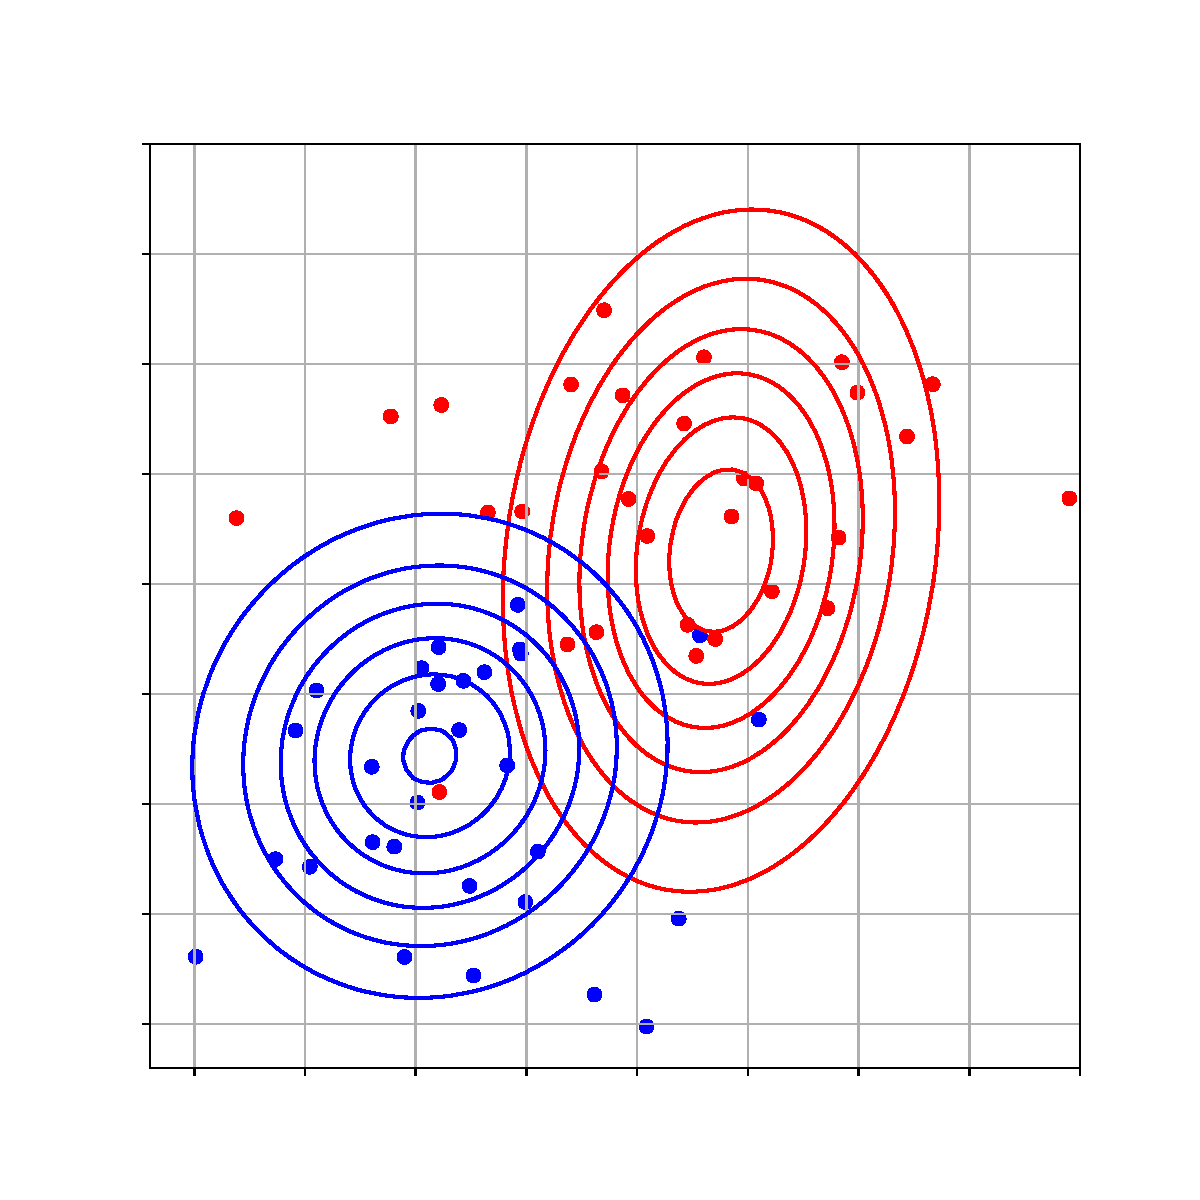
\includegraphics[width=\textwidth]{figures/normal_class}
        \label{fig:udp_header}
        \caption{A normal classifier}
    \end{subfigure}
    %
    \centering
    \begin{subfigure}{0.4\textwidth}
        \centering
        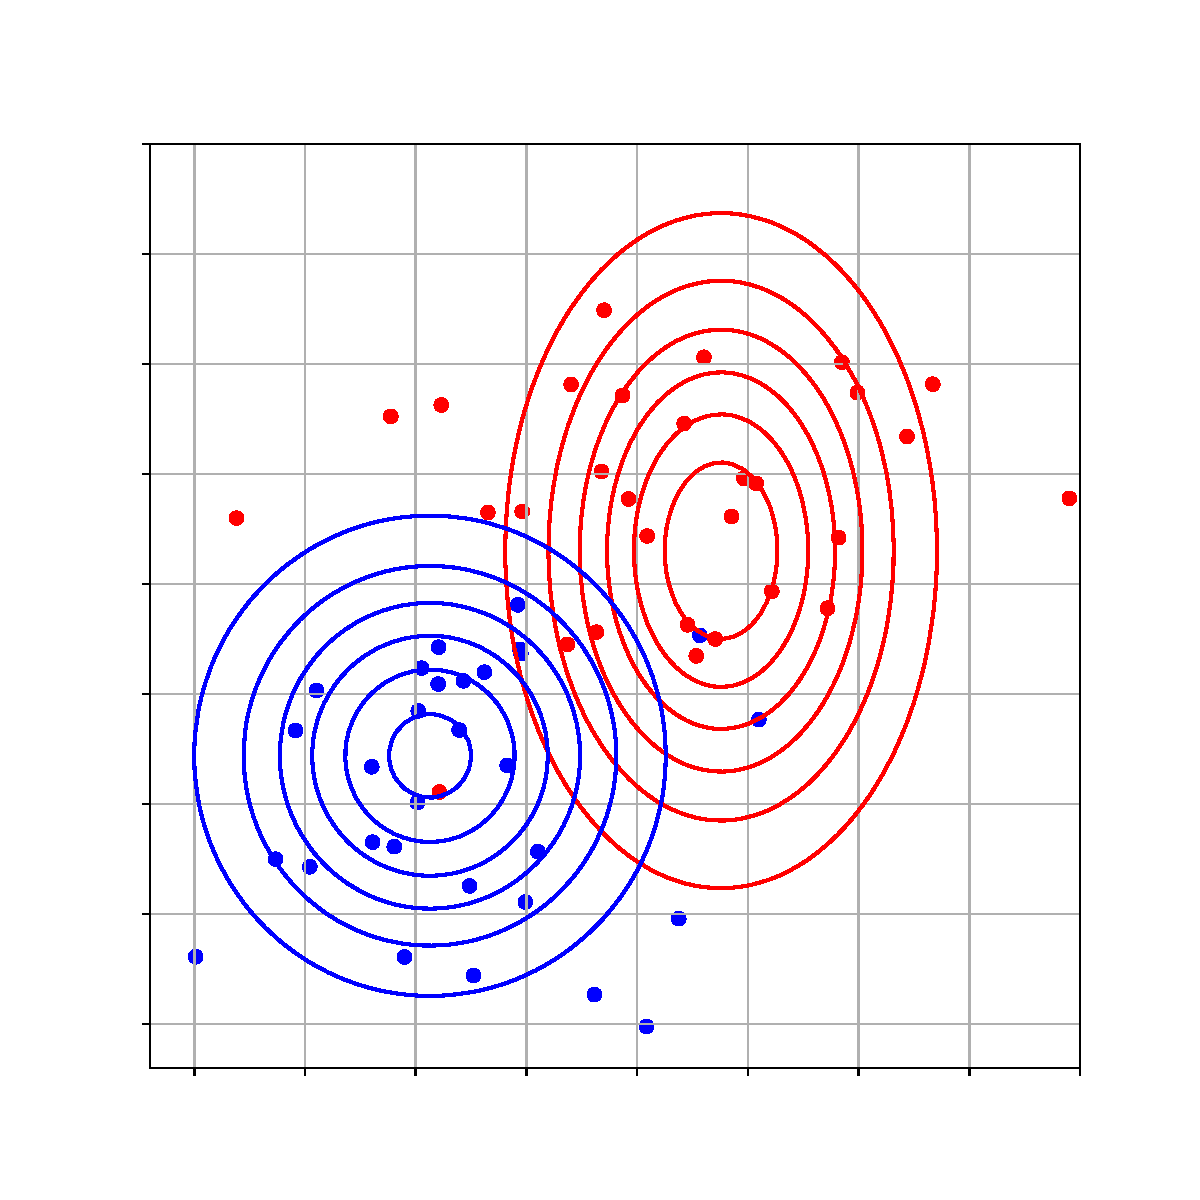
\includegraphics[width=\textwidth]{figures/normal_class_naive}
        \label{fig:tcp_header}
        \caption{A "naive" normal classifier. The multivariate Gaussian has no diagonal covariance, hence it can only stretch, but not rotate.}
    \end{subfigure}
\end{figure}

\section{Logistic Regression}
\subsection{Gradient Descent}
From the chain rule, we have $\frac{dw}{dt} = w_x \frac{dx}{dt} + w_y \frac{dy}{dt} + w_z \frac{dz}{dt}$. In vector notation, this becomes $\frac{dw}{dt} = \nabla w \cdot \frac{\vf{r}}{dt}$, where $\vf{r}$ is a curve in 3 dimensions. Thus:

\begin{equation*}
    \nabla w = \langle w_x, w_y, w_z \rangle
\end{equation*}

The gradient vector's values depend on the point where we evaluate it. It is also perpendicular to a level surface $w = c$ by the following proof:
\vskip 0.1in

Proof: For any curve $\vec{r} = \vec{r}(t)$ that is inside the level surface $w = c$, the velocity is in the tangent plane. This follows from the fact that derivatives are tangents to the function curve from 1-D calculus. Then by the chain rule above $\frac{dw}{dt} = \nabla w \cdot \frac{\vec{r}}{dt} = \frac{c}{dt} = 0$. Hence the gradient is perpendicular to the surface.
\vskip 0.1in

\textbf{Directional derivatives}. These are derivatives in the direction of some vector $\hat{\mathbf{u}}$. Treat $\frac{\partial w}{\partial x}$ as the derivative along the $x$-axis. In other words, this is a slice of the function as given by the $x$-plane. Now let's have a curve $\vec{r}(t)$, such that it has a \textit{normal} velocity $\hat{\mathbf{u}} = \langle a, b \rangle$. We can assume $|\hat{\mathbf{u}}| = 1$, since we are only interested in the direction. In other words:

\begin{equation*}
    \begin{cases}
        x(s) &= x_0 + as \\
        y(s) &= y_0 + bs
    \end{cases}
\end{equation*}

Now $s$ is the change in the direction of the curve. We can ask then what $\frac{\partial w}{\partial s}$ is. Well, by the chain rule:

\begin{equation*}
    \frac{\partial w}{\partial s} = \nabla w \cdot \frac{d\vf{r}}{ds} = \nabla w \cdot \hat{\mathbf{u}}
\end{equation*}

But from algebra we know:

\begin{equation*}
    \frac{\partial w}{\partial s} = \nabla w \cdot \hat{\mathbf{u}} = |\nabla w| |\hat{\mathbf{u}}| \cos{\theta} = |\nabla w| \cos{\theta}
\end{equation*}

This is maximized when $\cos{\theta} = 1$, i.e. when the gradient $\hat{\mathbf{u}}$ is in the direction of $\nabla w$. Hence the gradient points to the direction of steepest increase.

\subsection{So what?}
Patience. This can be applied to machine learning with the following idea. We normally define a loss or cost function $L$ (or $J$ as often seen in statistics). This is a function of our weights/ parameters. We usually aim to minimize said cost function. Well, if we know the direction of its steepest increase, $\nabla_{\vf{w}} L$, we know the direction of its steepest decrease - $-\nabla_{\vf{w}} L$. Hence we can take small steps in that direction:

\begin{equation*}
    \vf{w} \leftarrow \vf{w} - \eta \nabla_{\vf{w}}
\end{equation*}

\subsection{Logistic Regression.. finally}
\begin{figure}
    \centering
    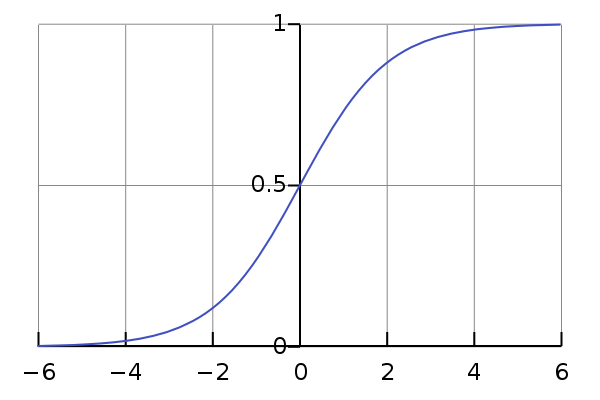
\includegraphics[width=0.4\textwidth]{figures/600px-Logistic-curve.png}
    \caption{Logistic Sigmoid (from wikipedia)}
    \label{fig:sigmoid}
\end{figure}

We want to classify things, which we can interpret as computing the probability $P(y = 1 | \bx, \bw)$. Enter the sigmoid:

\begin{equation*}
    f(\vf{x}; \vf{w}) = \sigma(\vf{w}^T \vf{x}) = \frac{1}{1 + e^{\vf{w}^T \vf{x}}}
\end{equation*}

See \autoref{fig:sigmoid}. We also need to define our loss function. We define another \textbf{super-duper important} concept in ML - the likelihood of the data given the weights:

\begin{align*}
    \text{Likelihood} &= P(\mathcal{D} | \vf{w}) = 
        P(\vf{x}^{(1)}, y^{(1)}, \dots, \vf{x}^{(N)}, y^{(N)}\ |\ \vf{w}) \\
    &= \underbrace{\prod_i P(\vf{x}^{(i)}, y^{(i)} |\ \vf{w})}_{\text{\blue{independent x's}}} = \prod_i P(y^{(i)} |\ \vf{x}^{(i)}, \vf{w}) P(\vf{x}^{(i)}\ |\ \vf{w}) \\
    &= \prod_i P(y^{(i)} |\ \vf{x}^{(i)}, \vf{w}) \underbrace{P(\vf{x}^{(i)})}_{\text{\blue{ignore weights}}} = \prod_i P(y^{(i)} |\ \vf{x}^{(i)}, \vf{w})
\end{align*}

We \blue{ignore the weights}, since our model doesn't tell us anything about the input distribution. I.e. no matter the weights, the probability of having $\bx$ will remain $1$. Another way of saying this is that our model is \textbf{discriminative} as opposed to \textbf{generative}. We don't "generate" anything, everything has a probability $1$ of being generated. \footnote{\textit{I know this is sloppy but I've looked and I haven't found a better (mathematically rigorous) explanation for this. Suggestions are welcome.}}
\vskip 0.1in

We often minimize the negative \textbf{log-likelihood}, in this case primarily because it transforms the product into a sum. With some careful math, we can calculate it and fit logistic regression models.

\subsection{Softmax Regression}
If there are $K$ classes, we can one-hot encode them as:

\begin{equation*}
    \vf{y} = [0\ 0\ 0\ \dots\ 0\ 1\ 0\ \dots\ 0]
\end{equation*}

where we have a $1$ for the target class. We fit $K$ weights, $\vf{w}^{(k)}$, such that our output contains $K$ probabilities, for each class:

\begin{equation*}
    f_k = \frac{
        {e^{(\vf{w}^{(k)})}}^T \vf{x}
    }{
        \sum_{k'} {e^{(\vf{w}^{(k')})}}^T \vf{x}
    }
\end{equation*}

where we normalize by the sum of all outputs so that we get a proper probability distribution. We can use batch gradient descent to minimize the negative log-likelihood. The likelihood would be the following then:

\begin{align*}
    \nabla_{\vf{w}}^{(k)}\ \text{LL} &= \nabla_{\vf{w}^{(k)}} \log \prod P(y_c = 1\ |\ \vf{x}, W) \\
            &= \sum_n \nabla_{\vf{w}^{(k)}} \log P(y_c = 1\ |\ \vf{x}, W) \\ 
            &= \sum_n (\vf{y}_k^{(n)} - f_k(\vf{x}^{(n)})) \vf{x}^{(n)}
\end{align*}

\subsection{Robust Regression}
Sometimes we get outliers in the data we cannot filter in the pre-processing stage. We assume that for each observation there is a probability it isn't part of the data. Or, in math terms:

\begin{equation*}
    P(m)\ =\ \text{Bernoulli}(m; 1 - \epsilon) =
        \begin{cases}
            1 - \epsilon & \text{m = 1} \\
            \epsilon     & \text{m = 0}
        \end{cases}
\end{equation*}

then we pick a random label when $m = 0$:

\begin{equation}
    P(y = 1\ |\ \vf{x}, \vf{w}, m) =
        \begin{cases}
            \sigma(\vf{w}^T\vf{x}) & m = 1 \\
            \frac{1}{2}              & m = 0
        \end{cases}
\end{equation}

The likelihood for a single example becomes:

\begin{align*}
    P(y = 1\ |\ \vf{x}, \vf{w}) &= \sum_m 
        P(y = 1, m\ |\ \vf{x}, \vf{w}) \\
    &= \sum_m P(y = 1\ |\ \vf{x}, \vf{w}, m) P(m) \\
    &= (1 - \epsilon) \sigma(\vf{w}^T\vf{x}) + \frac{\epsilon}{2}
\end{align*}

We can then derive the gradient for this and maximize the likelihood. We can treat $\epsilon$ as a hyperparameter and optimize over a validation set or set $\epsilon = \sigma(b)$ and optimize $b = \text{logit}(\epsilon) = \log \frac{\epsilon}{1 - \epsilon}$.


\section{Neural Networks}
\label{sec:nn_intro}
\textit{This section is taken from by Bachelor's thesis, so it might not read very well in a summary kind of way.}
\vskip 0.1in

Neural networks are universal function approximators inspired by biological neurons (e.g. \cite[Chapter~6]{goodfellow_deep_2016}). The main building blocks of neural networks are called \textit{neurons} and the networks are often drawn as directed graphs, as in figure \ref{fig:neural_net}. This graph illustrates the \textit{flow} of the network, from the \textit{inputs} $x_1, x_2, x_3$ to the \textit{output} $y$. Each circle in the figure is called a neuron and each of the three vertical slices is called a layer. The layers that are not the input or output layers are called \textit{hidden} layers.

\begin{figure}
    \centering
    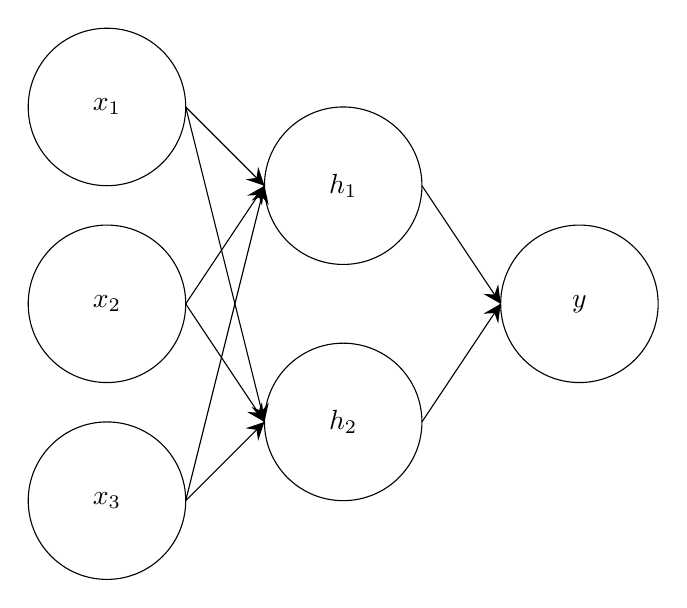
\begin{tikzpicture}
        \tikzset{myptr/.style={decoration={markings,mark=at position 1 with %
        {\arrow[scale=2,>=stealth]{>}}},postaction={decorate}}}
    
        % left row
        \draw (0, 0) circle (1) node {$x_3$};
        \draw (0, 2.5) circle (1) node {$x_2$};
        \draw (0, 5) circle (1) node {$x_1$};
        
        % middle row
        \draw (3, 1) circle (1) node {$h_2$};
        \draw (3, 4) circle (1) node {$h_1$};
        
        % right row
        \draw (6, 2.5) circle (1) node {$y$};
        
        % lines
        % to h_2
        \draw[myptr] (1, 0) -- (2, 1);
        \draw[myptr] (1, 2.5) -- (2, 1);
        \draw[myptr] (1, 5) -- (2, 1);
        % to h_1
        \draw[myptr] (1, 0) -- (2, 4);
        \draw[myptr] (1, 2.5) -- (2, 4);
        \draw[myptr] (1, 5) -- (2, 4);
        % to y
        \draw[myptr] (4, 1) -- (5, 2.5);
        \draw[myptr] (4, 4) -- (5, 2.5);
    \end{tikzpicture}
    
    \caption[Neural network example]{Neural Network illustration. The inputs are $x_1, x_2, x_3$, the hidden layers are $h_1, h_2$ and $y$ is the output.}
    \label{fig:neural_net}
\end{figure}


In what is called the \textit{supervised learning} scenario, the neural network is trained to predict the outputs $y$ given the inputs $\mathbf{x}$ (see next section). If $y$ is real-valued, then the task is called \textit{regression} and is what we will attempt to do in the context of ABC.
\vskip 0.1in

We can define the transformations equivalently from the inputs to the hidden layer and from the hidden units to output(s) via a system of equations:
%
\begin{align}
    \mathbf{h} &= W^{(1)}\ \mathbf{x} \\
    y &= W^{(2)}\ \mathbf{h}
\end{align}

Thus we can increase or decrease the size of the input vector in subsequent layers of the network depending on the shapes of the  matrices $W^{(1)}$ and $W^{(2)}$.
\vskip 0.1in

We apply a piecewise non-linearity called the \textit{activation function} after each matrix multiplication, i.e. at each neuron; without it, the model could be collapsed to a single layer:

\begin{align}
    \mathbf{h} &= h^{(1)}(W^{(1)}\ \mathbf{x}) \\
    y &= h^{(2)} (W^{(2)}\ \mathbf{h})
\end{align}

Choices for activation functions $h(\mathbf{x})$ include hyperbolic tangent ($\tanh$), sigmoids ($\sigma(x)$) and rectified linear units (relu):

\begin{align}
    \text{tanh}(x) &= \frac{e^x - e^{-x}}{e^x + e^{-x}} \\
    \sigma(x) &= \frac{1}{1 + e^{-x}} \\
    \text{relu}(x) &= \text{max}(0, x)
\end{align}

Additionally, parametric rectifier units allow the activation to be non-zero (and hence, the derivative as well):

\begin{equation}
    \text{prelu}(x) = \begin{cases}
        x       & \text{if}\ x > 0 \\
        a\ x    & \text{otherwise}
    \end{cases}
\end{equation}

The parameter $a$ is learned akin to the rest of the neural network parameters.
\vskip 0.1in

Rectified (and parametric) linear units generally learn faster than $\tanh$ and sigmoid units and are preferred in state-of-the-art applications \citep{glorot_deep_2011}. One improvement we will make is to replace the previously used $\tanh$ activations with relu units.
\vskip 0.1in

We can think of the hidden layers of the network as \textit{learned} feature transformations. If the outputs $y$ are real-valued and unbounded, i.e.\ in a regression task, we normally use a linear activation for the final layer, so we can think of the outputs from the previous hidden layer as features or \textit{basis} functions for the linear output neuron.

\begin{equation}
    y = W^{{K - 1}}\ \mathbf{h}^{(K - 1)}
\end{equation}

where we have K layers, including the output.

\subsection{Training Neural Networks}
\label{sec:nn_train}

To train the neural network, we use \textit{backpropagation} \citep{rumelhart_learning_1985}. More specifically, we use more optimized versions of backpropagation, namely \textit{Adam} \citep{kingma_adam:_2014} and \textit{RMSProp} \citep{tieleman_t._and_hinton_g._e._lecture_2012}.
\vskip 0.1in

Before we train, we specify a \textit{loss function}. The loss function gives us a measure of "how bad" it is to differ from the true output $y$, where $\hat{y}$ is the output of the neural network. We then train on a set of examples $\{\mathbf{x}^{(i)}, \mathbf{y}^{(i)}\}_{i = 0}^{N}$ via backpropagation. For a regression task, we use the mean-squared error loss function:

\begin{equation}
    \mathcal{L}(y, \hat{y}) = \frac{1}{N} \sum_{i = 1}^{N} (y^{(i)} - \hat{y}^{(i)})^2
\end{equation}

Backpropagation computes the derivative of the weight matrices $W^{(i)}$ with respect to the loss function for a \textit{batch} of training examples from the training set. It then moves the weight in the direction of the negative gradient, thus minimizing the loss function. The backpropagation algorithm takes as a parameter a \textit{learning rate}, which can be optimized. There are also more advanced versions, which often perform better, such as Adam \citep{kingma_adam:_2014} and RMSProp \citep{tieleman_t._and_hinton_g._e._lecture_2012}.

\begin{algorithm}
    \caption{Basic Backpropagation Algorithm}
    \begin{algorithmic}[1]
        \State initialize learning rate $\eta$

        \While{Error is still high (see Early Stopping)}
            \State $\mathbf{w} \gets \mathbf{w} - \eta \nabla \mathbf{w}$
            \Comment Update weights
        \EndWhile
    \end{algorithmic}
\end{algorithm}

\subsection{Modern Deep Neural Networks}
\label{subsec:nn_modern}

Using the simple backpropagation algorithm and neural networks introduced so far does not scale well to larger models and datasets \citep[Chapter 7]{goodfellow_deep_2016}. We can employ a number of techniques to improve the learning procedure. We describe here Batch Normalization \citep{ioffe_batch_2015}, Early Stopping \citep{prechelt_early_2012} and Dropout \citep{srivastava_dropout:_2014}, as well as \textit{regularization} in general.
\vskip 0.1in

A problem with larger networks is \textit{overfitting}. Normally, we train the network on a training set and then evaluate the performance on a separate \textit{validation set}, unseen during training. If the network learned the underlying structure of the data, then we say it \textit{generalizes} and we expect the loss on the validation set to be comparable to that on the training set. Networks with more free parameters (weights) as compared to the number of training examples can, however, learn to "remember" quirks in the training instances instead of learning such an underlying structure. In this thesis, in the context of ABC, we have the benefit of procedurally generating the data, so we do not have issues with the number of examples; we can have as many as needed.
\vskip 0.1in

\textbf{Early Stopping} is a relatively easy way to prevent overfitting \citep{prechelt_early_2012}. Consider figure \ref{fig:overfitting}. The training error normally will approach a very small number if the model has enough capacity. The validation error, however, usually starts increasing after it reaches a (sometimes local) minimum. If we continue to train, we no longer learn useful information, but rather quirks in the training set. Thus early stopping monitors the validation error at each epoch and stops training if the validation error continues to \textit{increase} for a number of epochs. We then revert to the best epoch so far.
\vskip 0.1in

\textbf{Batch Normalization} forces the activations of different layers in the network to be normalized \citep{ioffe_batch_2015}. This has been shown to help with poor initialization strategies and large input values by forcing outputs of layers to take on the same distribution, thus helping learning. Using batch normalization after each (fully-connected) layer helps the network by eliminating the need to learn the different output distributions of each layer. The following transformation is used after applying the activation functions on each layer:

\begin{align}
    \hat{z}_i &= \frac{h_i - \mu_i}{\sqrt{\sigma_i^2 + \epsilon}} \\
    h_i &= \gamma_i\ \hat{z}_i + \beta_i
\end{align}

Here $h_i$ are the outputs of each hidden unit and $\mu_i$ and $\sigma_i$ are minibatch mean and standard deviation, computed over training examples. $\gamma_i$ and $\beta_i$ are \textit{learned} scaling parameters and $\epsilon$ is a small value to prevent division by 0.
\vskip 0.1in

\textbf{Dropout} is another simple regularization technique \citep{srivastava_dropout:_2014}, that can prevent overfitting. During training we disconnect each neuron with a certain probability. This forces the other neurons to learn when some of the features are not present, thus making the network more flexible. At test time all the neurons are used and the outputs are scaled accordingly.
\vskip 0.1in

\textbf{L2 Regularization} is another way to prevent overfitting. We add a penalty term to the loss function for the entire neural network consisting of the squared absolute value of the weights for each layer. This forces the weights of the network to be small, thus ensuring the gradient updates are also small. It also prevents the activations from \textit{exploding}.

\begin{equation}
    \mathcal{\hat{L}}(y, \hat{y}, \{W^{(i)}\}_{i = 1}^{K}) = \frac{1}{N} \sum_{i = 1}^{N} (y^{i} - \hat{y}^{i})^2 + \sum_{i,j,k} \lambda (W_{i,j}^{(k)})^2
\end{equation}

where $\lambda$ is the regularization strength.

\begin{figure}
    \centering
    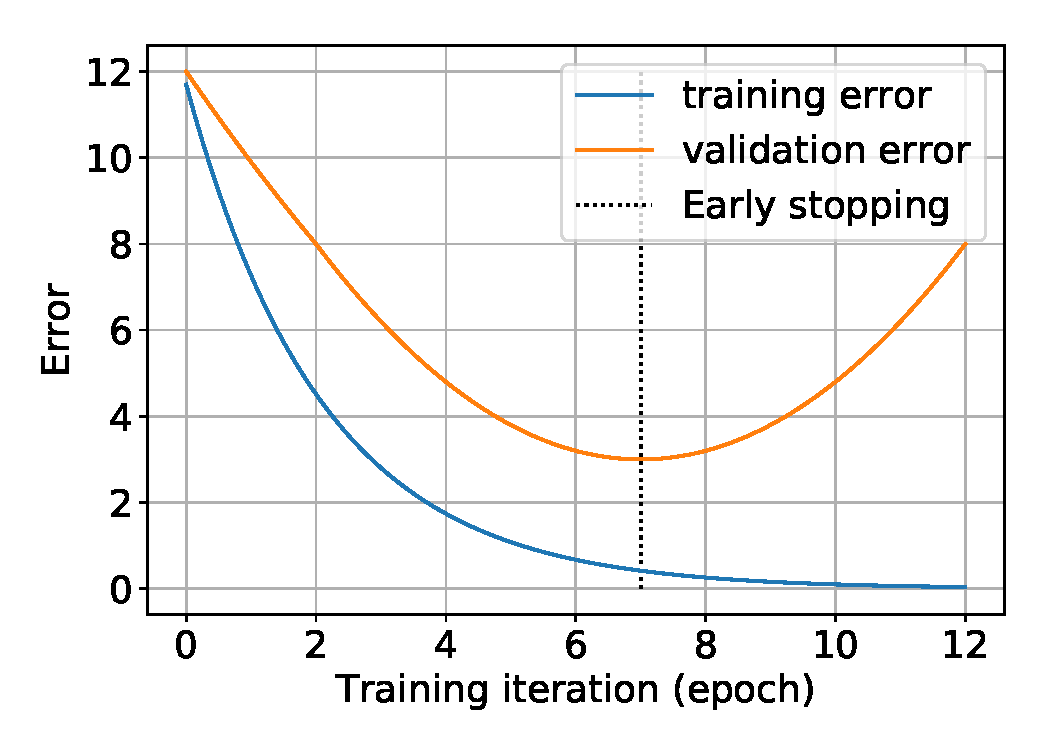
\includegraphics[width=0.7\textwidth]{figures/overfitting_early_stopping}
    \caption[Overfitting illustration]{Neural Network overfitting illustration. The training error almost reaches $0$, but the validation error starts to increase as the networks begins to learn structure present \text{only} in the training set.}
    \label{fig:overfitting}
\end{figure}

\textbf{Note} for all neural network models used in this thesis both the input data and the targets were standardized. This helps learning by avoiding large values for any neuron and therefore large gradients that become unstable:

\begin{equation}
    \hat{x}\ =\ \frac{x - \langle x \rangle}{\sqrt{\text{Var}[x]}}
\end{equation}

\section{Autoencoders and PCA}
\subsection{Autoencoders}
Autoencoders learn transformations or representations of data. The basic idea is to create a bottleneck somewhere in the middle of the network so that networks learn to represent the data in a smaller number of dimensions. Thus autoencoders are functions that return the input approximately:

\begin{equation}
    f(\bx) \approx \bx
\end{equation}

We can use a neural network with a hidden size less than the input, like so:

\begin{align*}
    \vf{h} &= g^{(1)}(W^{(1)} \bx + \vf{b}^{(1)}) \\
    \vf{f} &= g^{(2)}(W^{(2)} \vf{h} + \vf{b}^{(1)}) \\
\end{align*}

where $W^{(1)}$ is $K \times D$ and $K << D$. We can additionally impose a regularization penalty to further constrain the network. Sparse autoencoders, for instance, impose an L1 regularization. More about why that drives weights to zero below.
\vskip 0.1in

Denoising autoencoders learn to reconstruct the data when some of the inputs are missing or swapped or with added noise. Those are useful for removing noise from real-world images. 

\subsection{Principal Component Analysis (PCA)}
We compute the covariance matrix of the data $\Sigma = \frac{1}{N} X^T X$. We want to reduce dimensionality (from $D$ to $K$) in a way that maximizes the variance along the $K$ new axis. This can be done by computing the eigenvectors of the covariance matrix and then projecting the data along those axis. These eigenvectors are also orthogonal to each other; if we keep all dimensions (i.e. project onto all eigenvectors), no information is lost. This process is also equivalent to a linear autoencoder with a square loss function (TODO: proof).
\vskip 0.1in

Often we standardize the data (i.e. $\frac{x - \mu}{\sigma}$) which means we can omit the ${1}{N}$ in the calculation above. 

\subsection{Singular Value Decomposition}
Or SVD decomposes an $N\times D$ matrix into a product of a $N\times K$ matrix $U$, a diagonal $K\times K$ matrix $S$ and $K\times D$ matrix $V^T$:

\begin{equation*}
    X \approx USV^T
\end{equation*}

The columns of $U$ contain the eigenvectors of $X X^T$ and the rows of $U$ and the columns of $V^T$ give $K$-dimensional embeddings of the rows and columns of $X$, respectively.

\subsection{Probabilistic PCA}
We want to embed the data $X = \{\vf{x}^{(n)}\}$ into a $K$-dimensional space, such that $K < D$. Let's assume that each point is embedded into a latent variable $\vf{z}^{(n)}$. We assume that the latent variables are normally distributed:

\begin{equation*}
    \vf{z}^{(n)} \sim \mathcal{N}(\vf{0}, \mathbb{I})
\end{equation*}

We also assume that the original data is generated via a projection:

\begin{equation}
    \vf{x}^{(n)}\ |\ \vf{z}^{(n)} \sim \mathcal{N}(W\vf{z}^{(n)}, \sigma^2 \mathbb{I})
\end{equation}

where the matrix $W$ is $D\times K$. $\sigma$ is known as the noise term. We are interested in estimating $W$ and $\sigma$. Marginalizing out the $\vf{z}^{(n)}$, we arrive at:

\begin{equation}
    \vf{x}^{(n)} \sim \mathcal{N}(\vf{0}, WW^T + \sigma^2 \mathbb{I})
\end{equation}

This is then fitted via e.g. maximum likelihood.

\section{Bayesian Modeling}
We can adopt a probabilistic model for regression. Our training data consists of pairs $(\bx, y)$. We can assume a simple model:

\begin{equation*}
    P(y\ |\ \bx, \bw) = \mathcal{N}(y; f(\bx, \bw), \sigma_y^2)
\end{equation*}

where $f(\bx, \bw)$ is any function. A quadratic regression would have a quadratic expansion, for example. We can then fit using maximum likelihood or in practice by minimizing the negative log-likelihood:

\begin{align*}
    - \log P(\by \giv X, \bw) &= - \sum_n logP(y^{(n)} \giv \bx^{(n)}, \bw) \\
        &= \frac{1}{2 \sigma_y^2} \sum_n \big[  (y^{(n)} - f(\bx^{(n)}, \bw)) \big] + \frac{N}{2} \log(2 \pi \sigma_y^2)
\end{align*}

which is equivalent to fitting by least squares. Neat.

\section{Bayesian Regression}
\begin{figure}
    \centering
    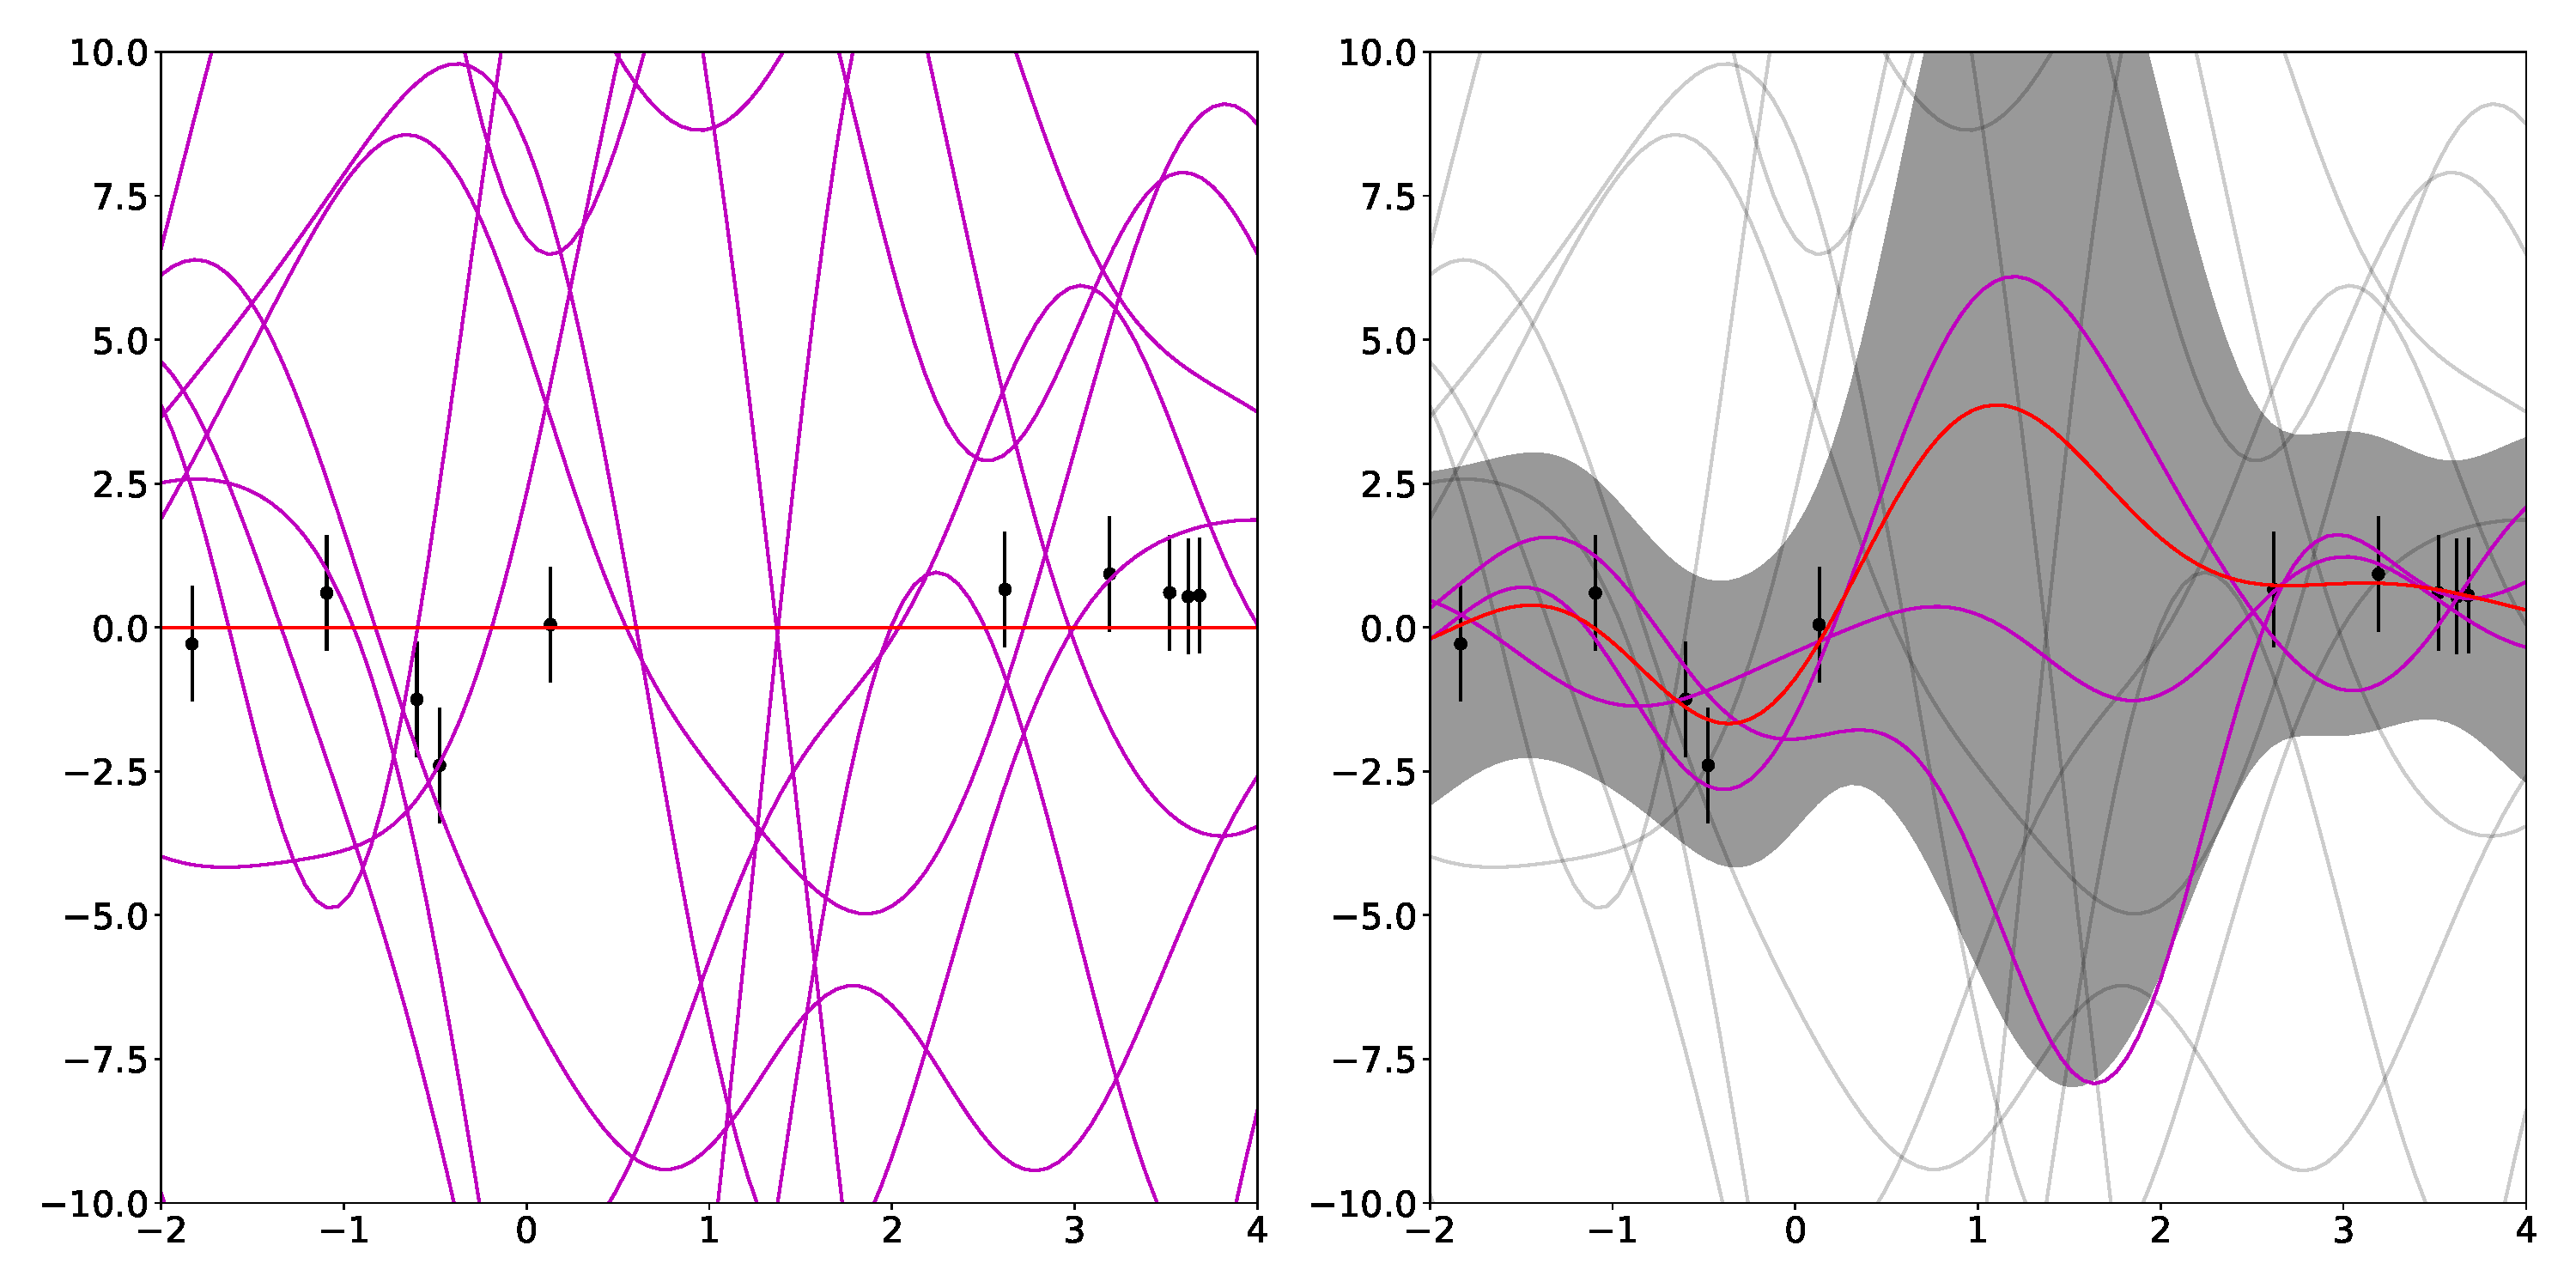
\includegraphics[width=0.8\textwidth]{figures/bayes_regression}
    \caption{Example Bayesian Regression with basis functions. The left graph has fits sampled from the prior. The shaded region in the right graph is centered at the posterior mean with one standard deviation plotted. The red line is the mean fit. The bars on each datapoint represent the noise $\sigma_y$.}
    \label{fig:bayes_regression}
\end{figure}

We need to set-up two things - a probabilistic model, like the one above, and a prior belief for our model. A simple way to do this would be as follows:

\begin{align*}
    P(\bw) &= \mathcal{N}(\bw; \vf{0}, \sigma_w^2 \mathbb{I}) \\
    P(y\ |\ \bx, \bw) &= \mathcal{N}(y; \bw^T \phi(\bx^{(n)}), \sigma_y^2)
\end{align*}

where this is a linear regression and $\phi(\bx^{(n)})$ represents any transformation we can apply. We can thus compute our posterior beliefs about the weights $\bw$ given our training examples (using Bayes' theorem, of course):

\begin{align*}
    P(\bw \giv \mathcal{D}) &\propto P(\mathcal{D} \giv \bw) P(\bw) \\
        &\propto \mathcal{N}(\bw; \vf{0}, \sigma_w^2 \mathbb{I})
            \prod_n \mathcal{N}(y^{(n)}; \bw^T \phi(\bx^{(n)}), \sigma_y^2) \\
        &\propto \mathcal{N}(\bw; \vf{0}, \sigma_w^2 \mathbb{I})\ 
            \mathcal{N}(\by; \Phi \bw, \sigma_y^2 \mathbb{I})
\end{align*}

This is also a Gaussian and can be derived (Murphy). If $\bw_0 = \bf{0}$ for the prior and $V_0 = \sigma_w^2 \mathbb{I}$, then:

\begin{align*}
    V_n &= \sigma_y^2(\sigma_y^2 V_0^{-1} + \Phi^T \Phi)^{-1} \\
    \bw_n &= V_n V_0^{-1} \bw_0 + \frac{1}{\sigma_y^2} V_N \Phi^T \by
\end{align*}

where $\bw_N$ is the posterior mean and $V_n$ - the posterior covariance.

\subsection{Test Predictions}
So we have our posterior $\bw$. Now we want, conditioned on the training data $\mathcal{D} = \{\bx^{(n)}, y^{(n)}\}$ to give predictions for a new test point $\bx^*$ with output $y^*$. We introduce our weights using the sum rule:

\begin{equation*}
    P(y^* \giv \bx^*, \mathcal{D}) = \int P(y^*, \bw \giv \bx^*, \mathcal{D}) \ \de\bw
\end{equation*}

Now we split the above using the product rule:
\begin{align*}
    P(y^* \giv \bx^*, \mathcal{D}) &= \int P(y^* \giv \bw, \bx^*, \mathcal{D})
        \ P(\bw \giv \bx^*, \mathcal{D}) \ \de\bw \\
    &= \int P(y^* \giv \bw, \bx^*)\ 
        P(\bw \giv \mathcal{D}) \ \de\bw
\end{align*}

where $\bw$ does not depend on the test input $\bx^*$. The test prediction also doesn't depend on the training data if we know $\bw$, the parameters. Now, we know the posterior for $\bw$:

\begin{equation*}
    P(\bw \giv \mathcal{D}) = \mathcal{N}(\bw; \bw_N, V_N)
\end{equation*}

For linear models the above integral is Gaussian. Expecting that, we can write:

\begin{align*}
    y^* &= f(\bx^*) + \nu = \bw^T \bx^* + \nu \\
    \nu &\sim \mathcal{N}(0, \sigma_y^2)
\end{align*}

This matches what we previously descibed as:

\begin{equation*}
    P(y^* \giv \bw) = \mathcal{N}(y^*; \bw^T \bx^*, \sigma_y^2)
\end{equation*}

We can thus show that:

\begin{equation*}
    P(y^* \giv \mathcal{D}, \bx^*) =
        \mathcal{N}(y^*; \bw_N^T \bx^*, (\bx^*)^T V_n \bx^* + \sigma_y^2)
\end{equation*}

\subsection{Decision Making}
The above answer is a distribution of $y^*$. Sometimes we need to ouput a single prediction, a guess. Thus we need to write a loss function $L(y, y^*)$, which says how bad it is to guess $y^*$ if the actual output is $y$. We can compute the expected loss:

\begin{equation*}
    c = \mathbb{E}_{P(y \giv \mathcal{D})}[L(y, y^*)] =
        \int L(y, y^*)\ P(y \giv \mathcal{D})\ \de y
\end{equation*}

For square loss, $L(y, y^*) = (y - y^*)^2$, we can differentiate the cost $c$ with respect to our guess:

\begin{equation*}
    \frac{\partial c}{\partial y^*} =
        \mathbb{E}_{P(y \giv \mathcal{D})} \frac{\partial L(y, y^*)}{\partial y^*} =
        \mathbb{E}_{P(y \giv \mathcal{D})} [2(y - y^*)] =
        2 (\mathbb{E}_{P(y \giv \mathcal{D})} [y] - y^*)
\end{equation*}

Setting this to $0$, the optimal guess is the posterior mean, $y^* = \mathbb{E}_{P(y \giv \mathcal{D})}[y]$. Thus if we only need the guess, using Bayesian regression does not change much at all. In fact this can be shown to correspond to a L2-regularized standard linear regression.

\section{Bayesian Logistic Regression}
For logistic regression, the likelihood function (as above) is defined as:

\begin{align*}
    P(\mathcal{D} \giv \model) &=  P(\data \giv \bw) =
        P(\vf{x}^{(1)}, y^{(1)}, \dots, \vf{x}^{(N)}, y^{(N)}\ |\ \vf{w}) \\
    &= \underbrace{\prod_i P(\vf{x}^{(i)}, y^{(i)} |\ \vf{w})}_{\text{\blue{independent x's}}} = \prod_i P(y^{(i)} |\ \vf{x}^{(i)}, \vf{w})\ P(\vf{x}^{(i)}\ |\ \vf{w}) \\
    &= \prod_i P(y^{(i)} |\ \vf{x}^{(i)}, \vf{w}) \underbrace{P(\vf{x}^{(i)})}_{\text{\blue{ignore weights}}} = \prod_i P(y^{(i)} |\ \vf{x}^{(i)}, \vf{w})
\end{align*}

When fitting via maximum likelihood, we do something like:

\begin{equation*}
    \bw^* = \argmax_{\bw} [ \log\ P(\by \giv X, \bw) -  \bw^T \bw ]
\end{equation*}

or, as most optimizers are optimized for minimizing functions, equivalently minimize the negative log-likelihood. Bayesian logistic regression begins the same way as Bayesian linear regression:

\begin{equation*}
    P(\bw \giv \data) = \frac{P(\data \giv \bw) P(\bw)}{P(\data)} \propto P(\data \giv \bw) P(\bw)
\end{equation*}

To make predictions (for a datapoint $y^*, \bx^*$), we can use probability theory:

\begin{align*}
    P(y^* \giv \bx^*, \data) &= \int P(y^*, \bw \giv \bx^*, \data) \de\bw \\
        &= \int P(y^* \giv \bx^*, \bw) P(\bw \giv \data) \de\bw
\end{align*}

The problem, of course, is that we can't really compute the posterior $P(\bw \giv \data)$. It never really is Gaussian as it were in the linear regression case. Thus we must be clever. In reality, if we assume a Gaussian prior, then posterior is this:

\begin{align*}
    P(\bw) &= \normal(\bw; \mathbf{0}, \sigma_w^2 \mathbb{I}) \\
    P(\bw \giv \data) &= \normal(\bw; \mathbf{0}, \sigma_w^2 \mathbb{I})
        \prod_n \sigma(\bw^T \bx^{(n)} z^{(n)})
\end{align*}

where $z^{n} = \{ +1, -1 \}$ instead of $\{0, 1\}$. If we notice that $\sigma(-a) = 1 - \sigma(a)$, then the above follows. Either way, this product of sigmoids and a Gaussian is nasty and very slow to integrate numerically above. We can do importance sampling to predict like so:

\subsection{Importance Sampling}
\begin{figure}
    \centering
    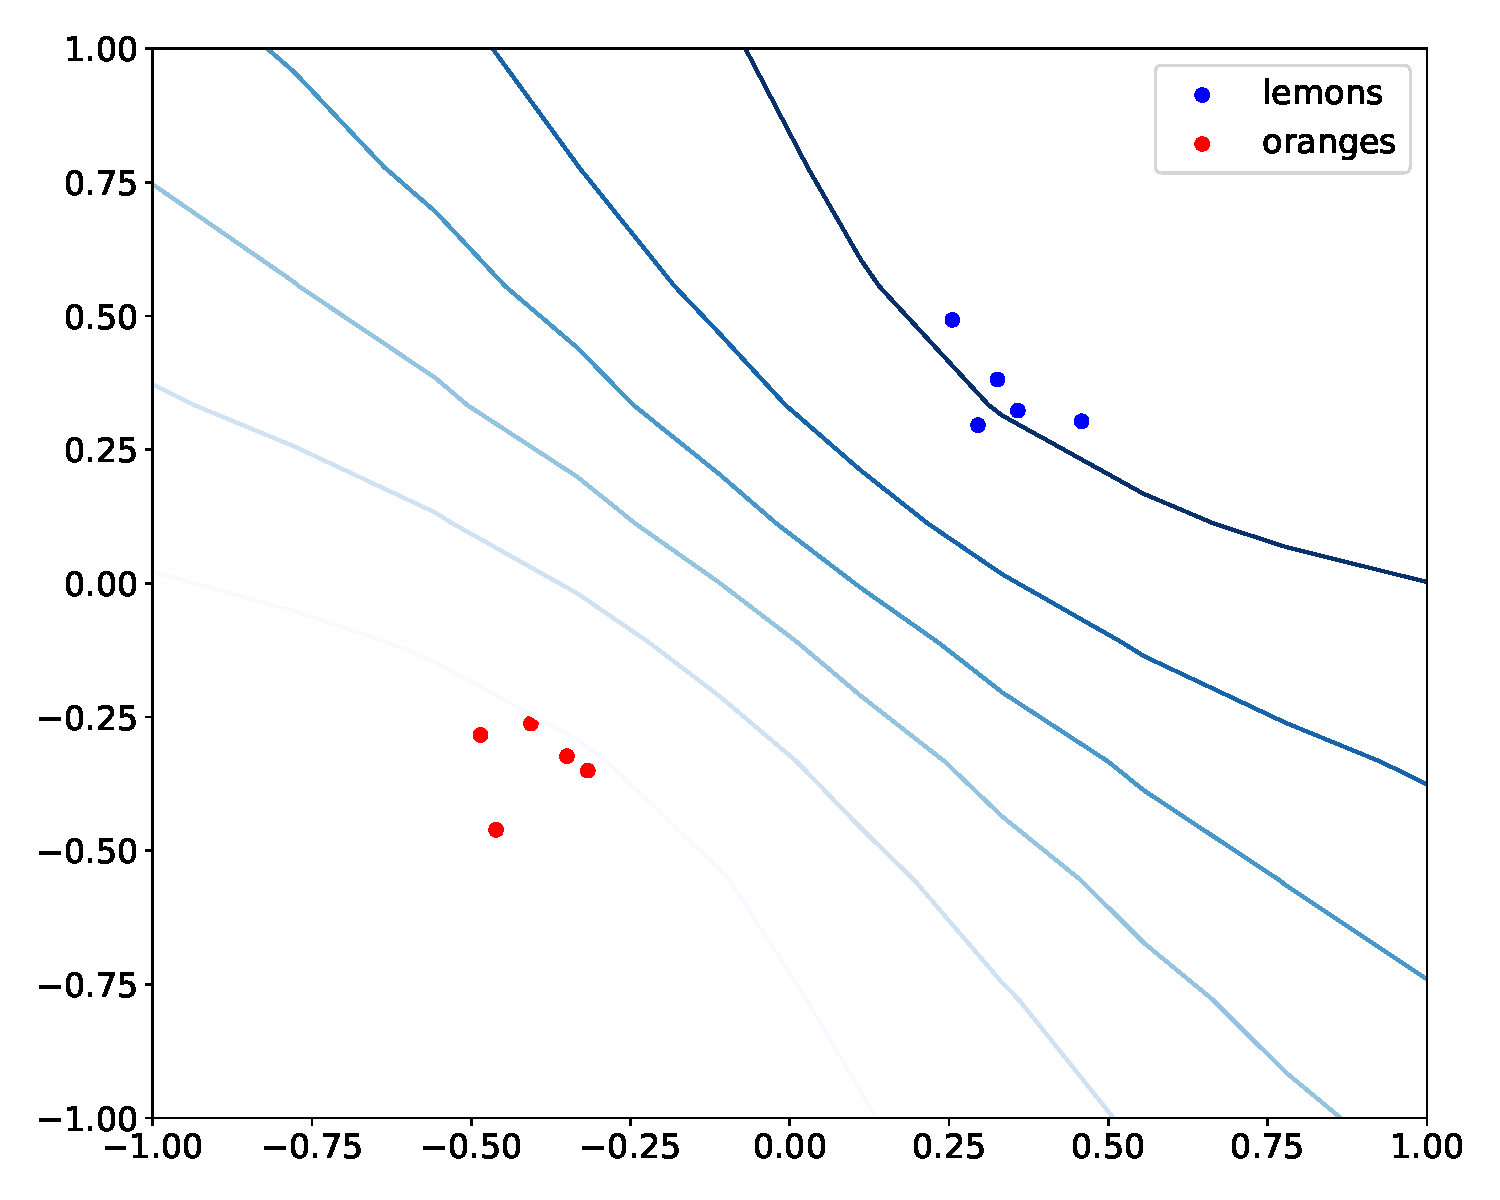
\includegraphics[width=0.6\textwidth]{figures/bayes_logistic}
    \caption{Bayesian Logistic Regression via Importance Sampling}
    \label{fig:bayes_log_importance}
\end{figure}

\begin{align*}
    P(y^* \giv \bx^*, \data) &= \mathbb{E}_{P(\bw \giv \data)}[P(y^* \giv \bx^*, \bw)] \\
        &\approx \frac{1}{S} \sum_{s = 1}^{S} P(y \giv, \bx^*, \bw^{(s)})
\end{align*}

where $\bw^{(s)} \sim P(\bw \giv \data)$. Sampling from the posterior $P(\bw \giv \data)$ is hard. We can do many things, like MCMC, but perhaps the easiest is importance sampling:

\begin{align*}
    P(y^* \giv \bx^*, \data) &= \int P(y^* \giv \bx^*, \bw) P(\bw \giv \data)\ \de\bw \\
        &= \int P(y^* \giv \bx^*, \bw) \frac{P(\data \giv \bw) P(\bw)}{P(\data)}\  \de\bw \\
    &= \mathbb{E}_{P(\bw)} [P(y^* \giv \bx^*, \bw) \frac{P(\data \giv \bw)}{P(\data)}] \\
    &= \mathbb{E}_{P(\bw)} [P(y^* \giv \bx^*, \bw) \frac{P(\data \giv \bw)}{\int P(\data \giv \bw) P(\bw)\ \de\bw}] \\
    &= \mathbb{E}_{P(\bw)} [P(y^* \giv \bx^*, \bw) \frac{P(\data \giv \bw)}{\mathbb{E}_{P(\bw)}[P(\data \giv \bw)]}]
\end{align*}

Now we can do importane sampling in the denominator and in the entire expression, perhaps even storing samples from $P(\bw)$, the prior. The end result looks like this:

\begin{align*}
    P(y^* \giv \bx^*, \data) &\approx
        \frac{1}{S} \sum_s P(y^* \giv \bx^*, \bw^{(s)}) \frac{
            P(\data \giv \bw^{(s)})
        }{
            \frac{1}{S'} \sum_{s'} P(\data \giv \bw^{(s')})
        }
\end{align*}

where $w^{(s)} \sim P(\bw)$. The bias of this, of course, is humongous. \autoref{fig:bayes_log_importance} shows an example result of this procedure.
\vskip 0.1in

Another thing we can do is:

\subsection{Maximum a Posteriori}
which is just this:

\begin{equation*}
    \bw^* = \argmax_\bw[\log P(\bw \giv \data)] =
        \argmax_\bw[\log P(\data \giv \bw) P(\bw)]
\end{equation*}

c.f. maximum likelihood. Really we only added the prior here. Onwards to:

\subsection{Laplace Approximation}
Let's assume that the posterior $p(\bw \giv \data)$ is Gaussian. That's not a very good assumption, putting it mildly. We can try matching the best Gaussian to it. We first find the maximum likelihood, the most probable value of $\bw$, which we label $\bw^*$, as usual:

\begin{align*}
    \bw^* &= \argmax_\bw P(\bw \giv \data) \\
        &= \argmax_\bw\ \log \frac{P(\data, \bw)}{P(\data)} \\
        &= \argmax_\bw\ \log P(\data | \bw) P(\bw)
\end{align*}

The last line follows from the fact that $P(\data)$ is independent of $\bw$, i.e. a constant in the optimization problem. We also can't really evaluate $P(\data)$, since it's a nasty integral. So far, so good. We can define the energy as follows:

\begin{align*}
    E(\bw) &= -\log P(\bw, \data) \\
    \bw^* &= \argmin_\bw E(\bw)
\end{align*}

Then we compute the Hessian, the matrix of second derivatives. This gives us the curvature of the function:

\begin{equation*}
    H_{i, j} = \frac{
        \partial^2 E(\bw^*) 
    }{
        \partial w_i\ \partial w_j
    }
\end{equation*}

The energy of a Gaussian distribution would be, up to a constant:

\begin{equation*}
    E_\gauss (w) = \frac{(w - \mu)^2}{2\sigma^2}
\end{equation*}

The minimum is at $w^* = \mu$ and the second derivative - $H = 1 / \sigma^2$. Generalizing to a higher dimension, we get:

\begin{equation*}
    E_\normal(\bw) = \frac{1}{2} (\bw - \mathbf{\mu})^T \Sigma^{-1} (\bw - \mathbf{\mu})
\end{equation*}

where $\bw^* = \mathbf{\mu}$ and $H = \Sigma^{-1}$ or $\Sigma = H^{-1}$. Thus matching energies, we get:

\begin{equation*}
    P(\bw \giv \data) \approx \normal(\bw; \bw^*, H^{-1})
\end{equation*}

To approximate $P(\data)$, we can do:

\begin{align*}
    P(\bw \giv \data) &= \frac{P(\bw, \data)}{P(\data)}
        \approx \normal(\bw; \bw^*, H^{-1}) =
        \frac{|H|^{1/2}}{(2\pi)^{D/2}} \exp(-\frac{1}{2}
            (\bw - \bw^*)^{\text{T}} H (\bw - \bw^*)) 
\end{align*}

This is true for any $\bw$, so let's evaluate it for $\bw^*$, giving us:

\begin{align*}
    P(\bw \giv \data) &= \frac{P(\bw, \data)}{P(\data)}
        \approx \normal(\bw^*; \bw^*, H^{-1}) =
        \frac{|H|^{1/2}}{(2\pi)^{D/2}}
\end{align*}

which gives us:
\begin{equation*}
    P(\data) \approx P(\bw^*, \data)\ |2 \pi H^{-1}|^{1/2}
\end{equation*}

\subsection{Test Predictions}
For a test point $y^*, \bx^*$, we need to compute:

\begin{align*}
    P(y^* \giv \bx^*, \data) &= \int P(y^*, \bw \giv \bx^*, \data)\ \de\bw \\
    &= \int P(y^* \giv \bx^*, \bw)\ P(\bw \giv \data)\ \de\bw
\end{align*}

Using the Laplace approximation above, we know that $P(\bw \giv \data) \approx \normal(\bw; \bw^*, H)$, we have the following integral:

\begin{align*}
    P(y^* = 1 \giv \bx, \data) &\approx
        \int \sigma(\bw \bx^\text{T}) \normal(\bw; \bw^*, H^{-1})\ \de\bw \\
    &= \mathbb{E}_{\normal(\bw; \bw^*, H^{-1})} [\sigma(\bw \bx^\text{T})]
\end{align*}

Calling $a = \bw^* \bx^\text{T}$ and changing variables:

\begin{align*}
    P(a) &= \normal(a; \bw^* \bx^\tran, \bx^\tran H^{-1} \bx)\\
    P(y = 1 \giv \bx, \data) &= 
        \int \sigma(a)\ \normal(a; \bw^* \bx^\tran, \bx^\tran H^{-1} \bx) \ \de a
\end{align*}

which we can then compute numerically. From Murphy Section 8.4.4.2, we can derive another approximation:

\begin{align*}
    P(y = 1 \giv \bx, \data) &\approx \sigma(\kappa \bw^* \bx) \\
    \kappa &= \frac{
        1
    }{
        \sqrt{
            1 + \frac{\pi}{8} \bx^\tran V \bx
        }
    }
\end{align*}

\section{Optimizing Hyperparameters in a Bayesian Setting}
We normally opt to choose simpler models, that is models that assign a high probability to the training data, over models that have an high probability of generating many datasets. We can thus specify the probability:

\begin{align*}
    P(\data \giv \model) &= P(X, \by \giv \model) =
        P(\by \giv X, \model) \underbrace{P(X \giv \model)}_\text{\blue{1}} \\
    &= P(\by \giv X, \model) = \int P(\by, \bw \giv X, \model)\ \de\bw =
        \int P(\by \giv X, \bw, \model)\ P(\bw \giv \model)\ \de\bw
\end{align*}

The probability of the data given the model, i.e. $P(\data \giv \model)$ is the \textbf{marginal likelihood} of the model. We can use it to select between different models $\model_k$.
\vskip 0.1in

(\textit{Yet another example from MLPR}) If we have a linear model with:
\begin{align*}
    P(\bw \giv \sigma_w) &= \normal(\bw; \mathbf{0}, \sigma_w^2 \mathbb{I}) \\
    P(y \giv \bw, \sigma_y) &= \normal(y; \bw^\tran \bx, \sigma_y^2)
\end{align*}

We then fit $\sigma_w$ and $\sigma_y$ by maximizing the marginal likelihood:

\begin{equation*}
    P(\by \giv X, \sigma_w, \sigma_y) =
        \int P(\by \giv X, \bw, \sigma_y)\ P(\bw \giv \sigma_w)\ \de\bw
\end{equation*}

\section{Gaussian Processes}
\begin{figure}
    \centering
    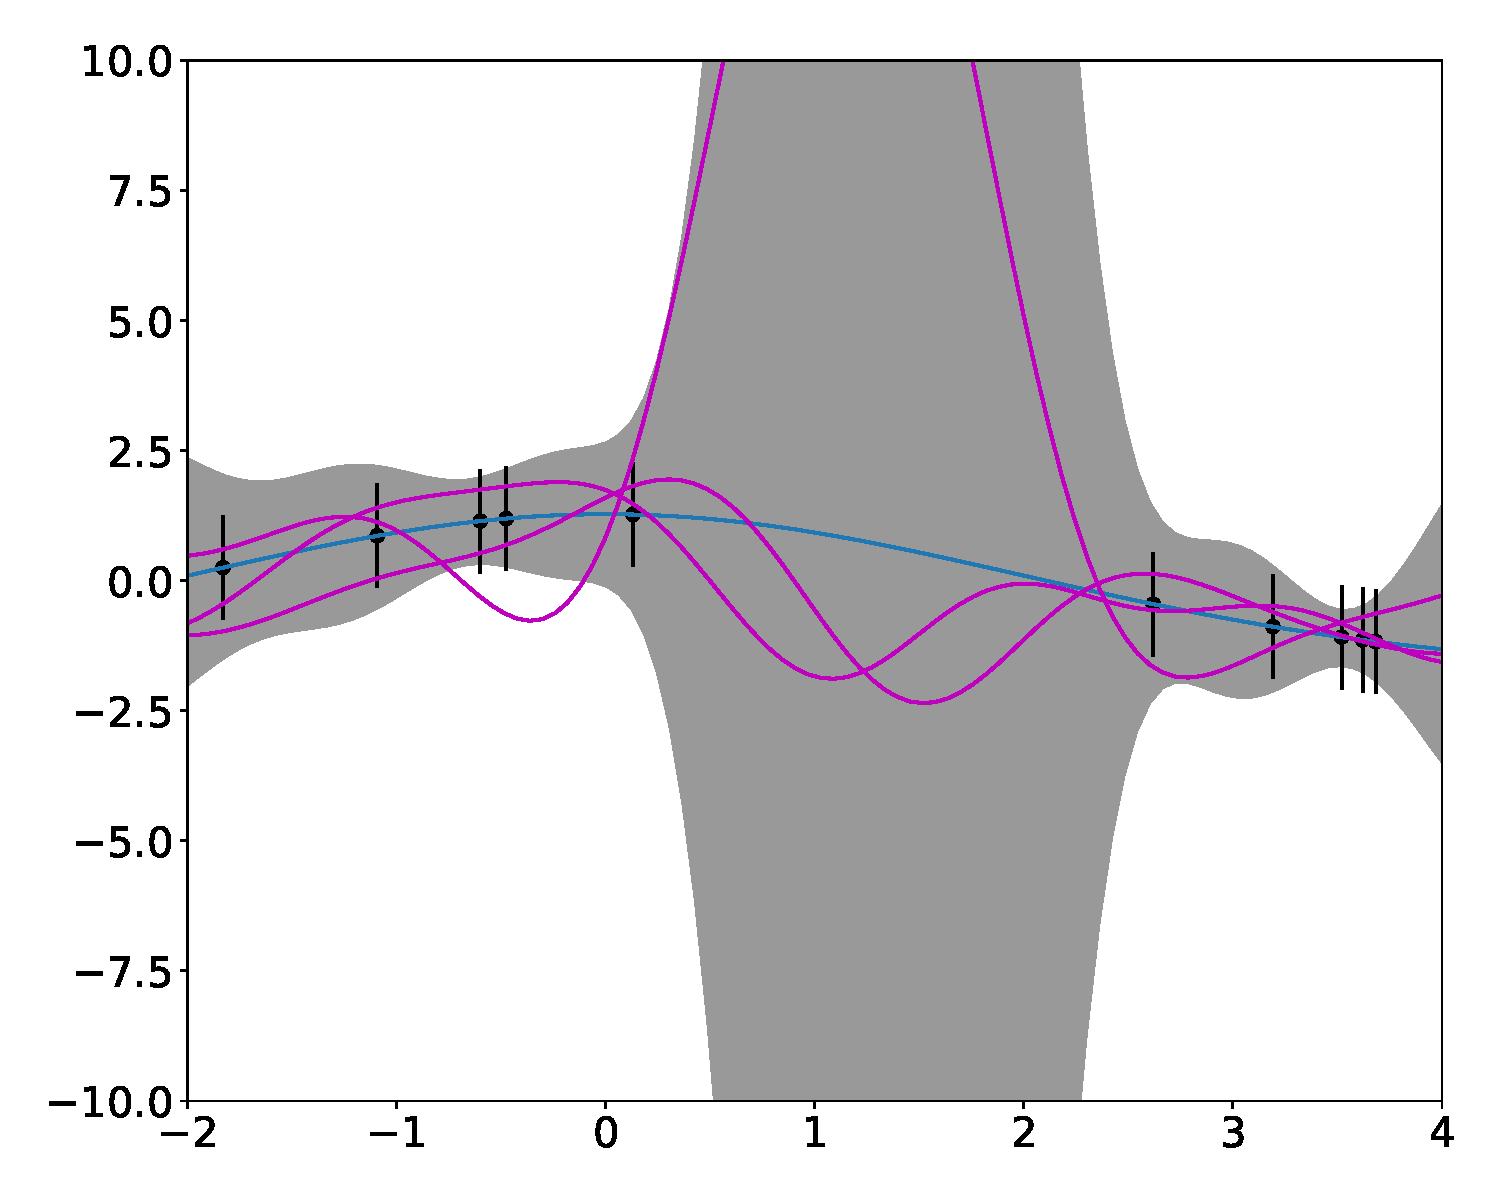
\includegraphics[width=0.6\textwidth]{figures/gp}
    \caption{Gaussian Process posterior}
    \label{fig:gp}
\end{figure}

Gaussian processes are just big Gaussians. Let's say we have a training set of values $\by$ and inputs $X$ and a test set of values (unknown) $\bfu_*$ and test inputs $X_*$. If we assume that everything comes from a Gaussian, i.e.:

\begin{equation*}
    P\bigg(\begin{bmatrix}
        \by \\
        \bfu_*
    \end{bmatrix}\bigg) = \normal\bigg(
        \begin{bmatrix}
            \by \\
            \bfu_*
        \end{bmatrix};
        \mathbf{0};
        \begin{bmatrix}
            K(X, X) + \sigma_y^2 \mathbb{I} & K(X, X_*) \\
            K(X_*, X) & K(X_*, X_*)
        \end{bmatrix}
    \bigg)
\end{equation*}

This really is the essence of the thing. The $K$ functions are the kernels that represent the covariance between datapoints. This is enough to describe any dataset; in fact a non-zero mean Gaussian process is always equivalent to a zero mean one (TODO: proof). The kernels are defined as:

\begin{equation*}
    K(X, Y)_{i, j} = k(\bx^{(i)}, \bz^{(j)})
\end{equation*}

for two test inputs $\bx$ and $\bz$. For training inputs we also have noise variance $\sigma_y^2$. Let's call the noise:

\begin{equation*}
    \nu_i \sim \normal(0, \sigma_y^2)
\end{equation*}

then for the cross-covariance:

\begin{align*}
    \text{cov}(y_i, f_{*, j}) &= \expect[y_i f_{*, j}] -
        \expect[y_i] \expect[f_{*,j}] \\
        &= \expect[(f_i + \nu_i) f_{*, j}] \\
        &= \expect[f_i f_{*,j}] + \underbrace{\expect[\nu_i]}_0\expect[f_{*, j}] \\
        &= \expect[f_i f_{*,j}] = k(\bx^{(i)}, \bx^{*, j})
\end{align*}

Once we specify the kernel $k$, we can extract the distribution of the test datapoints by simply marginalizing the big Gaussian:

\begin{align*}
    P(\bfu_* \giv \data, \model) =
        \normal&(\bfu_*; \\
        &K(X_*, X)(K(X, X) + \sigma_y^2 \mathbb{I})^{-1} \by, \\
        &K(X_*, X_*) - K(X_*, X)(K(X, X) + \sigma_y^2 \mathbb{I})^{-1}K(X, X_*) \\
        &)
\end{align*}

which is the posterior over test datapoints.

\subsection{Gaussian Kernel}
A common choice for a kernel is the Gaussian kernel:

\begin{equation*}
    k(\bx^{i}, \bx^{j}) = 
        \sigma_f^2 \exp\bigg( 
            -\frac{1}{2} \sum_{d=1}^D (x_d^{(i)} - x_d^{j})^2 /l_d^2    
        \bigg)
\end{equation*}

We can fit $\sigma_f$ and $\l_d$ by maximizing the marginal likelihood.

\section{Variational Inference}
Not going into details here. The idea is to minimize the Kullback-Leibler Divergence between two distributions. We can use it instead of the Laplace Approximation for Bayesian Logistic Regression above.

\begin{equation*}
    D_{KL}(p || q) = \int p(\bx) \log \frac{p(\bx)}{q(\bx)}\ \de\bx
\end{equation*}

We can minimize the KL divergence $D_{KL}(q(\bw; \alpha)\ ||\ P(\bw \giv \data))$ in the logistic regression case. We are trying to match a parametric function $p$ with some parameters captured in $\alpha$ to the posterior distribution of the weights $P(\bw \giv \data)$:

\begin{align*}
    \kl(q(\bw; \alpha)\ ||\ \post) &= \int q(\bw; \alpha) \log \frac{
        q(\bw; \alpha)
    }{
        \post
    }
    \ \de\bw \\
    &= -\int q(\bw; \alpha) \log \post\ \de\bw + 
    \underbrace{
        \int q(\bw; \alpha) \log q(\bw; \alpha)\ \de\bw
    }_{\text{negative entropy,} -H(q)}
\end{align*}

The first term is large if we put probability on regions where the posterior is small. The second term encourages more spread-out distributions with high entropy.
\vskip 0.1in

Using Bayes' theroem in the KL divergence formula:

\begin{equation*}
    \kl(q\ ||\ p) = \underbrace{
        \expect_q[\log q(\bw)] -
        \expect_q[\log P(\data \giv \bw)] -
        \expect_q[\log P(\bw)]
    }_{J(q)} + \log P(\data)
\end{equation*}

We thus minimize $J(q)$, also known as ELBO (Evidence Lower Bound). We can get a bound on the $P(\data)$ term, the marginal likelihood, by observing the KL divergence is non-negative:

\begin{equation*}
    \log P(\data) \geq -J(q)
\end{equation*}

\subsection{Minimizing the KL-divergence for a Gaussian function}
Let $\alpha = \{ \bm{m}, V \}$, the mean and co-variance of a Gaussian distribution. We will be (numerically) minimizing the $J(q)$ with respect to $\alpha$. Thus:

\begin{equation*}
    q(\bw; \alpha) = \normal(\bw; \bm{m}, V)
\end{equation*}

We first Cholesky decompose $V$ to get $V = LL^\tran$, $L$ being a lower-triangular matrix with positive diagonal entries. We also optimize $\log \sigma_w$; otherwise we might make $\sigma_w$ negative.

\begin{equation*}
    L = \begin{cases}
        \log L_{i, j} & i = j \\
        L_{i, j}      & i \neq j
    \end{cases}
\end{equation*}

We assume a Gaussian prior:

\begin{equation*}
    P(\bw) = \normal(\bw; \bf{0}, \sigma_w^2 \mathbb{I})
\end{equation*}

We can write two of the terms of $J(q)$ in closed form:

\begin{align*}
    \expect_{\normal(\bw; \bm{m}, V)}[\normal(\bw; \bmu, \Sigma)] &=
        \expect_{\normal(\bw; \bm{m}, V)}\bigg[
            -\frac{1}{2}(\bw - \bmu)^\tran \Sigma^{-1} (\bw - \bmu)
        \bigg] - \frac{1}{2} \log |2 \pi \Sigma] \\
    % 
    \expect_q[\log q(\bw)] &=
        \expect_{\normal(\bw; \bm{m}, V)}[\log \normal(\bw; \bm{m}, V)] = -\frac{D}{2} - \frac{1}{2}\log|2 \pi V| \\
    % 
    \expect_q[\log P(\bw)] &=
        \frac{1}{2\sigma_w^2}\bigg[ \text{Tr}(V) + \bm{m}^\tran \bm{m} \bigg] + \frac{D}{2} \log(2\pi\sigma_w^2)
\end{align*}

Using this trick:

\begin{align*}
    \expect_{\normal(\bz; 0, V)}[\log \normal(\bz; 0, V)] &=
        \expect[-\frac{1}{2} \text{Tr}(\bz^\tran V^{-1} \bz)]
    = -\frac{1}{2} \text{Tr}(\expect[\bz^\tran V^{-1} \bz])
    = -\frac{1}{2} \text{Tr}(\expect[\bz^\tran \bz] V^{-1}) \\
    &= -\frac{1}{2} \text{Tr}(VV^{-1}) = -\frac{1}{2} \text{Tr}(\mathbb{I}_D) = -\frac{D}{2}
\end{align*}

where $\expect[\bz^\tran \bz] = V$ by the definition of covariance for a $0$-mean random variable. We also know that $\bz^\tran V \bz$ is a number and hence equal to its trace, a.k.a. the "trace trick".
\vskip 0.1in

From the Cholesky decomposition:
\begin{align*}
    \frac{1}{2} \log|V| &= \sum_i \log L_{i,i} \\
    \text{Trace}(V) &= \sum_{i,j} L_{i,j}^2
\end{align*}

hence the above reparametrization.

\subsection{Log-likelihood term}
The nastiest of the three terms is the log-likelihood:

\begin{equation*}
    -\expect_{\normal(\bw; \bm{m}, V)}[\log P(\data \giv \bw)] =
        -\expect_{\normal(\bw; \bm{m}, V)}\bigg[
            \sum_{n=1}^N \log p(y^{(n)} \giv \bx^{(n)}, \bw)
        \bigg]
\end{equation*}

We cannot compute this in closed form. Instead we do a Monter Carlo estimate:

\begin{equation*}
    -\expect_{\normal(\bw; \bm{m}, V)}[\log P(\data \giv \bw)] \approx
        - \sum_{n = 1}^{N} \log p(y^{(n)}, \bx^{n}, \bw)
\end{equation*}

where $\bw \sim \normal{\bm{m}, V}$.

\subsection{Gradients of the log-likelihood}
Here we do a "reparametrization trick" (gotta love those). To sample a random $\bw$, we sample a vector of normal variables $\nu \sim \normal(0, \mathbb{I})$ and then transform it (see multivariate Gaussians above): $\bw = \bm{m} + L \nu$. We can rewrite the expectation:

\begin{equation*}
    \expect_{\normal(\bw; \bm{m}, V)}[f(\bw)] = \expect_{\normal(\pmb{\nu}; \bm{0}, \mathbb{I})}[f(\bm{m} + L \pmb{\nu})]
\end{equation*}

Now differentiating:
\begin{align*}
    \nabla_\bm{m} \expect_{\normal(\bw; \bm{m}, V)}[f(\bw)] &=
    \expect_{\normal(\pmb{\nu}; \bm{0}, \mathbb{I})}[\nabla_\bm{m} f(\bm{m} + L \pmb{\nu})] \\
    &\approx \nabla_\bm{m} f(\bm{m} + L \pmb{\nu}) \\
    % 
    \nabla_L \expect_{\normal(\bw; \bm{m}, V)}[f(\bw)] &=
    \expect_{\normal(\pmb{\nu}; \bm{0}, \mathbb{I})}[\nabla_L f(\bm{m} + L \pmb{\nu})] \\
    &\approx [\nabla_L f(\bw)]\pmb{\nu}^\tran
\end{align*}

\section{Gaussian Mixture Models}
This is a clustering algorithm. We have $K$ classes and each datapoint has a class: $z^{(n)} = \{1, \dots, K\}$. These are unobserved and drawn from a prior. $z^{(n)} \sim \pi$. The points come from the Gaussian mixtures:

\begin{equation*}
    P(\bx^{(n)} \giv z^{n} = k, \theta) = \normal(\bx^{(n)}; \pmb{\mu}^{(k)}, \Sigma^{(k)})
\end{equation*}

where $\theta = \{ \pi, \{ \bmu^{(k)}, \Sigma^{(k)} \}\}$. We can fit it via maximum likelihood by maximizing:

\begin{equation*}
    \log P(\data \giv \theta) = \sum_n \log P(\bx^{(n)} \giv \theta)
\end{equation*}

where:

\begin{align*}
    P(\bx^{(n)} \giv \theta) &=
        \sum_k P(\bx^{(n)}, z^{(n)} = k \giv \theta) \\
    &= \sum_k P(\bx^{(n)} \giv z^{(n)} = k, \theta) P(z^{(n)} = k \giv \theta) \\
    &= \sum_k \pi_k \normal(\bx^{(n)}; \bmu^{(k)}, \Sigma)
\end{align*}

We can't solve this analytically, but we can use gradient-based optimizers. We decompose $\Sigma = LL^\tran$ (Cholesky) and set:

\begin{equation*}
    L = \begin{cases}
        \log L_{i, j} & i = j \\
        L_{i, j}      & i \neq j
    \end{cases}
\end{equation*}

The $\pmb{\pi}$ vector must represent probabilities. We can use a softmax transformation.

\subsection{Expectation Maximization (EM)}
This consists of two steps, the $\bm{E}$ and $\bm{M}$ step:
\vskip 0.1in

$\bm{E}$-step:
\begin{equation}
    r_k^{(n)} = P(z^{(n)} = k \giv \bx^{(n)}, \theta) = \frac{
        \pi_k \normal(\bx^{(n)}; \bmu^{(k)}, \Sigma^{(k)})
    }{
        \sum_l \pi_l \normal(\bx^{(n)}; \bmu^{(l)}, \Sigma^{(l)})
    }
\end{equation}

$\bm{M}$-step:
\begin{align*}
    r_k = \sum_n r_k^{(n)}
    \pi_k &= \frac{r_k}{N} \\
    \bmu^{(k)} &= \frac{1}{r_k} \sum_n r_k^{(n)} \bx^{(n)} \\
    \Sigma^{(k)} &= \frac{1}{r_k} \sum_n r_k^{(n)} \bx^{(n)} \bx^{(n)\tran}
        - \bmu^{(k)} \bmu^{(k)\tran}
\end{align*}

% \section{Optimization}
% \subsection{Regularization in Depth}
% \subsection{Expectation Maximization}
% \subsection{Proximal Methods}

% \section{Ensembles}
% \subsection{Averaging}
% \subsection{Bagging}
% \subsection{Mixture of Experts}

\printbibliography

\end{document}
